\section{Conditional Use of Network State}
\label{sec:discount}

Given \S\ref{sec:rq2}, a natural next step is to discount the network term as its inputs age. We
built four such rules (Eqs.~\ref{eq:hard}--\ref{eq:channel}) and evaluated them in the same cells
as the two extremes (full trust $=$ NetworkAware2; no trust $=$ LeastLoad), ten seeds,
\num{12000} requests per cell, on all three workload sources. The comparison is paired
per-request within a cell, so it measures the rules rather than the configurations.

\subsection{What the first attempt got wrong (a falsified design)}
Our first design discounted \emph{within} the link term, on the hypothesis that a stale link
snapshot retains its structural content (``which link is wide'') while losing its dynamic content
(``who is congesting it now''): it kept the transfer term at full weight and decayed only the
congestion term. The hypothesis is mechanistically appealing and, on this evidence, wrong.
Table~\ref{tab:discount} shows what happened under a \SI{60}{\second}-old link snapshot: on the
Azure trace the term-split rule retains only $-40.2\%$ of the $-76.7\%$ available, whereas
applying a single factor to the whole network term retains $-76.2\%$. On the synthetic source it
is worse still ($+5.5\%$, i.e.~the benefit is destroyed entirely). The mechanism is the mirror
image of an earlier failure we made: muting the congestion penalty makes \emph{fat link, slow
compute} workers attractive again, and traffic piles onto exactly the worker the link term was
supposed to protect. \textbf{Discounting must be applied at the level of the information source
(the channel), not at the level of an individual score term.}

\begin{table*}[t]
\centering
\caption{Four discounting rules against the two extremes, under a \SI{60}{\second}-old link
snapshot with a fresh queue (all values are $\Delta$p95 vs.\ LeastLoad, \%; negative is better).
``per-channel'' is Eq.~\ref{eq:channel}, ``term-split'' is the falsified design
Eq.~\ref{eq:split}; ``uniform'' and ``hard'' are Eqs.~\ref{eq:linear} and~\ref{eq:hard}.
Values in parentheses are medians, given only where the trace batches' per-seed spread is large.}
\label{tab:discount}
\small
\setlength{\tabcolsep}{5pt}
\resizebox{\linewidth}{!}{%
\begin{tabular}{@{}llrrrrr@{}}
\toprule
Source & Cell & full trust & per-channel & term-split & uniform & hard \\
\midrule
Synthetic & d-heavy / degraded & $-68.2$ & $-61.2$ & $+5.5$ & $0.0$ & $0.0$ \\
Synthetic & mixed / degraded   & $-70.3$ & $-66.2$ & $-16.6$ & $0.0$ & $0.0$ \\
Azure     & d-heavy / degraded & $-76.7$ & $\mathbf{-76.2}$ & $-40.2$ & $+0.1$ & $+0.1$ \\
Azure     & mixed / degraded   & $-76.8$ & $\mathbf{-74.4}$ & $-31.1$ & $+0.7$ & $+0.5$ \\
BurstGPT  & mixed / degraded   & $-60.1$ & $-58.8$ & $-28.7$ & $-20.7$ & $-10.6$ \\
BurstGPT  & mixed / unstable, $5/60$\,s & $+32.5$ {\scriptsize$(+23.4)$} & $\mathbf{+3.0}$ {\scriptsize$(-0.1)$} & $+1.7$ & $-3.3$ & $+2.5$ \\
\bottomrule
\end{tabular}%
}
\end{table*}

\subsection{What the corrected rule buys, and what it does not}
\begin{figure}[t]
\centering
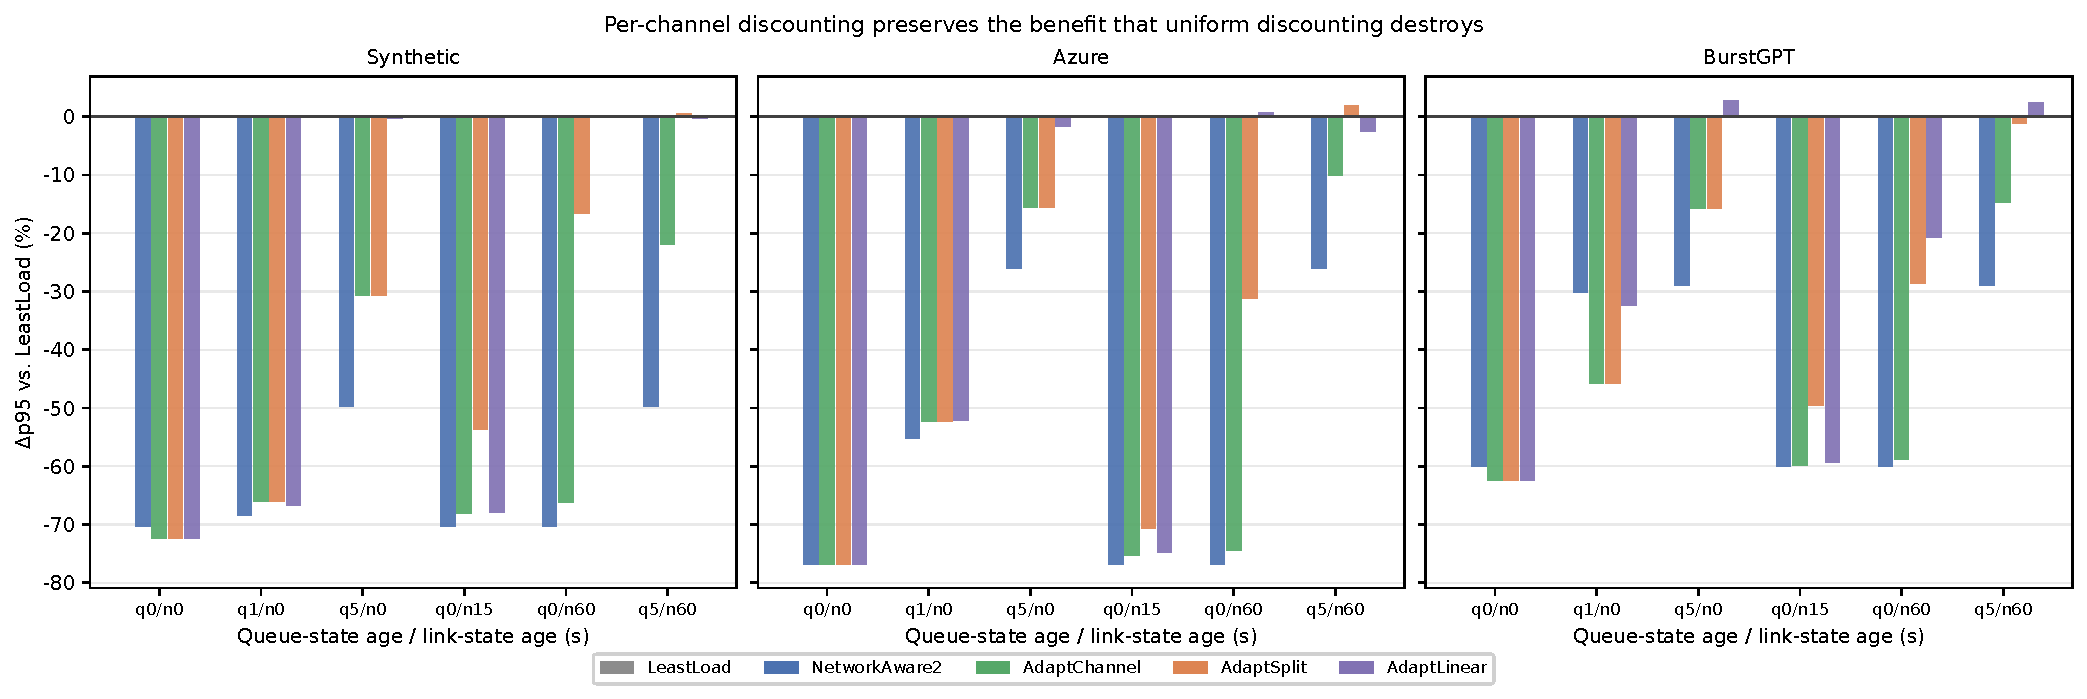
\includegraphics[width=\columnwidth]{fig_discount_rules}
\caption{The four discounting rules against both extremes, on the three workload sources
(mixed workload, heterogeneous static network). Per-channel discounting tracks full trust where
the link snapshot is old, while uniform and threshold discounting collapse to the network-blind
baseline.}
\label{fig:discount}
\end{figure}
The per-channel rule keeps $90$--$99\%$ of the available benefit under a \SI{60}{\second}-old
link snapshot on all three sources (Azure: $-76.7\%\rightarrow-76.2\%$; synthetic:
$-68.2\%\rightarrow-61.2\%$; BurstGPT: $-60.1\%\rightarrow-58.8\%$), where the uniform and hard
alternatives destroy \emph{all} of it. Figure~\ref{fig:discount} shows all four rules against both extremes on all three workload sources. In the language of \S\ref{sec:rq2}, this is expected: the
link channel's value barely decays, so \emph{any} discount applied to it mostly subtracts value.

The rule is not free, and we report where it loses (Table~\ref{tab:verdict}). It is a net loss in
the majority of conditions on the Azure source, and it never dominates the two extremes; what it
buys is the absence of a specific failure mode. That failure mode is visible in the last row of
Table~\ref{tab:discount}: on the burstiest source, with both channels stale, full trust is
\emph{harmful} (median $+23.4\%$, i.e.~the network-aware policy is worse than the policy that
ignores the network in the majority of seeds), and the per-channel rule removes that harm
(median $-0.1\%$). We emphasize that we found this only after replacing the mean of per-seed
relative differences with its median: the mean at that cell is $+32.5\%$ while the median is
$+23.4\%$ (both harmful, so the conclusion is robust \emph{here}), but at a neighbouring cell
(data-heavy/unstable, $5/0$) the mean is $+27.8\%$ while the median is $-0.5$ --- a
single-seed artifact that a mean-only table would have promoted to a finding.

\begin{table}[t]
\centering
\caption{Verdict counts over 24 conditions per source (6 staleness configurations $\times$ 2
workloads $\times$ 2 network conditions). ``Better than both'' counts conditions where the rule
beats \emph{both} full trust and no trust. No rule dominates.}
\label{tab:verdict}
\footnotesize
\setlength{\tabcolsep}{4pt}
\begin{tabular}{@{}lrrrrr@{}}
\toprule
Source & Rule & beats both & loses both & beats full & loses full \\
\midrule
\multirow{4}{*}{Synthetic} & per-channel & 5 & 1 & 5 & 18 \\
                           & term-split  & 4 & 3 & 4 & 19 \\
                           & uniform     & 5 & 5 & 5 & 18 \\
                           & hard        & 5 & 1 & 5 & 17 \\
\midrule
\multirow{4}{*}{Azure}     & per-channel & 1 & 4 & 1 & 22 \\
                           & term-split  & 1 & 5 & 1 & 22 \\
                           & uniform     & 2 & 4 & 4 & 19 \\
                           & hard        & 4 & 8 & 7 & 15 \\
\midrule
\multirow{4}{*}{BurstGPT}  & per-channel & 8 & 2 & 10 & 13 \\
                           & term-split  & 6 & 2 & 8 & 15 \\
                           & uniform     & 10 & 4 & 10 & 13 \\
                           & hard        & 7 & 3 & 8 & 14 \\
\bottomrule
\end{tabular}
\end{table}

\subsection{When is discounting actually needed?}
The robust way to ask this is not ``how large is the effect'' but ``in how many independent seeds
does full trust lose to the network-blind baseline''. Table~\ref{tab:seedcount} answers it, and
the answer is sharply localized. With a fresh queue, full trust wins in $9$--$10$ of $10$ seeds
even when the link snapshot is \SI{60}{\second} old --- discounting there is pure loss. On the
\emph{volatile} network with a \SI{5}{\second}-old \emph{queue}, full trust loses in 4--6 of 10
seeds on all three sources. That single cell is where discounting has a job to do, and it is
exactly the regime that the two-channel expiry model of \S\ref{sec:rq2} predicts.

\begin{table}[t]
\centering
\caption{Seeds (of 10) in which full trust beats the network-blind baseline. The only regime
where full trust is unreliable is a stale queue on a volatile network.}
\label{tab:seedcount}
\footnotesize
\setlength{\tabcolsep}{3pt}
\begin{tabular}{@{}llrrr@{}}
\toprule
Queue / link age & Source & mixed / deg. & mixed / unst. & d-heavy / unst. \\
\midrule
$0/60$\,s & Synthetic & 10 & 10 & 10 \\
$0/60$\,s & Azure     & 10 & 9  & 10 \\
$0/60$\,s & BurstGPT  & 10 & 9  & 6  \\
\midrule
$5/0$\,s  & Synthetic & 10 & 6  & 10 \\
$5/0$\,s  & Azure     & 10 & 4  & 4  \\
$5/0$\,s  & BurstGPT  & 8  & 7  & 5  \\
\bottomrule
\end{tabular}
\end{table}

\subsection{Parameter sensitivity}
\begin{figure}[t]
\centering
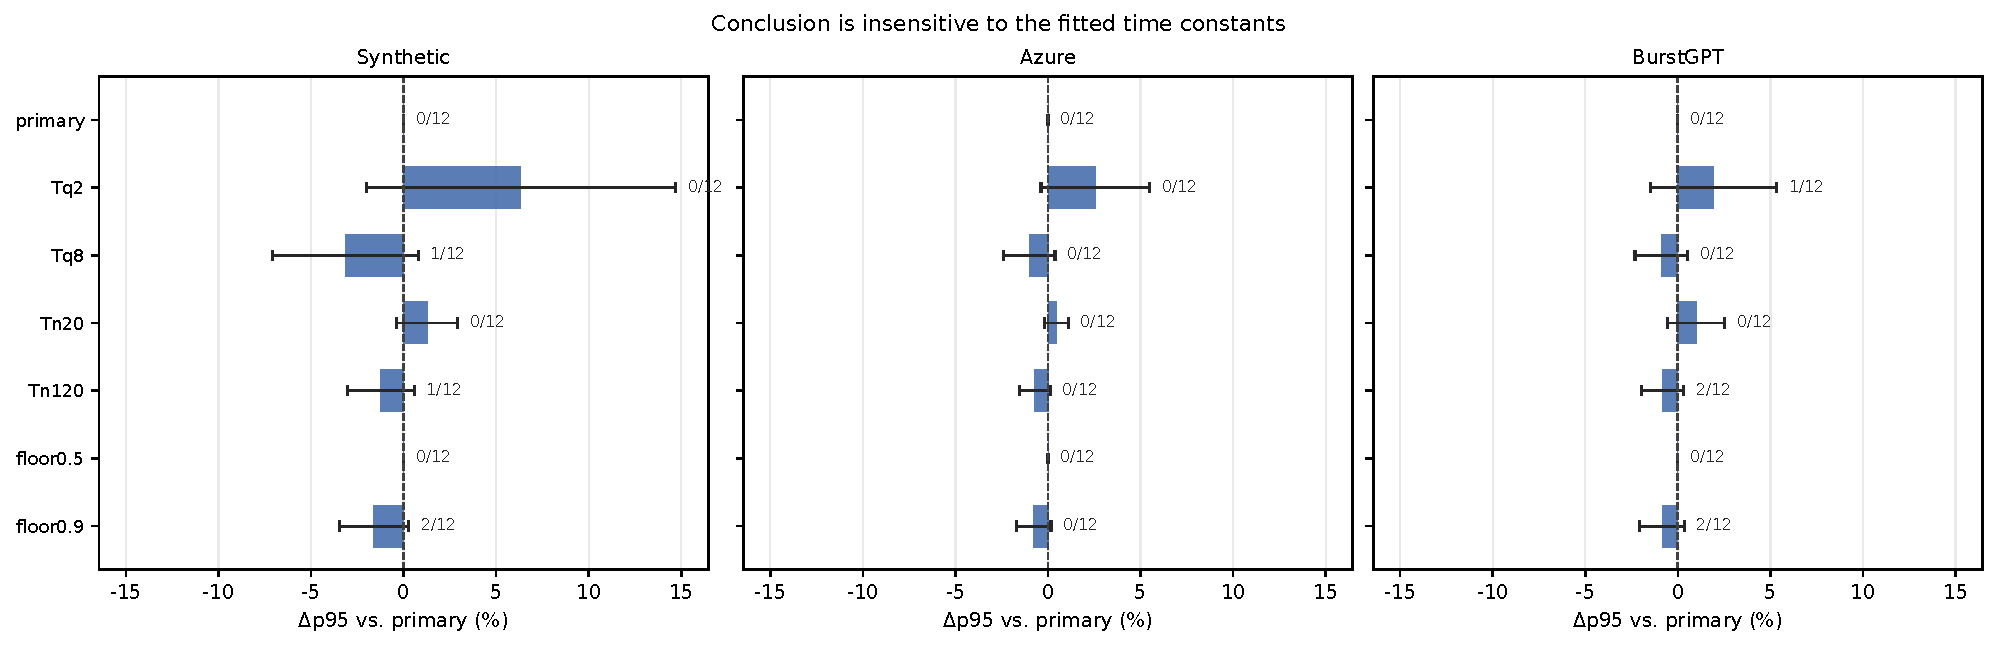
\includegraphics[width=\columnwidth]{fig_ablation}
\caption{One-factor-at-a-time ablation of the per-channel rule on all three sources. Bars show
the mean change in p95 relative to the unmodified rule with $95\%$ confidence intervals; the
annotation on each bar counts conditions where the sign of the conclusion changes.}
\label{fig:ablation}
\end{figure}
The rule of Eq.~\ref{eq:channel} has exactly three numbers, all read off the measured curves of
\S\ref{sec:rq2} rather than tuned. We ablate each by a factor of two, one at a time, on all three
sources (Table~\ref{tab:ablation}). Moving the link-side time constant between \SI{20}{\second}
and \SI{120}{\second} changes p95 by $-1.2$ to $+1.3\%$; moving the weight floor between $0.5$
and $0.9$ changes it by $-1.6$ to $0.0\%$; moving the queue-side constant between \SI{2}{} and
\SI{8}{\second} changes it by $-3.2$ to $+6.3\%$, with the confidence interval spanning zero. The
\emph{direction} of the conclusion (does the rule beat full trust?) flips in at most 2 of 12
conditions on any source, and in 0 of 12 on Azure. Figure~\ref{fig:ablation} summarizes the ablation across sources. The parameters are therefore not load-bearing individually
individually, which is what one wants from constants that are supposed to be read off data.

\begin{table}[t]
\centering
\caption{One-factor-at-a-time ablation of the per-channel rule (mean $\Delta$p95 vs.\ the
unmodified rule, with 95\% CI over 12 conditions; ``flips'' counts conditions where the
sign of ``rule vs.\ full trust'' changes).}
\label{tab:ablation}
\footnotesize
\setlength{\tabcolsep}{4pt}
\begin{tabular}{@{}lrrrr@{}}
\toprule
Variant & Synthetic & Azure & BurstGPT & flips (max) \\
\midrule
$\tau_q: 4\rightarrow2$\,s & $+6.3\pm8.4$ & $+2.6\pm2.9$ & $+1.9\pm3.4$ & 1/12 \\
$\tau_q: 4\rightarrow8$\,s & $-3.2\pm3.9$ & $-1.0\pm1.4$ & $-0.9\pm1.4$ & 1/12 \\
$\tau_n: 60\rightarrow20$\,s & $+1.3\pm1.7$ & $+0.4\pm0.6$ & $+1.0\pm1.5$ & 0/12 \\
$\tau_n: 60\rightarrow120$\,s & $-1.2\pm1.8$ & $-0.7\pm0.8$ & $-0.8\pm1.1$ & 2/12 \\
floor: $0.7\rightarrow0.5$ & $0.0\pm0.0$ & $0.0\pm0.0$ & $0.0\pm0.0$ & 0/12 \\
floor: $0.7\rightarrow0.9$ & $-1.6\pm1.9$ & $-0.8\pm0.9$ & $-0.9\pm1.2$ & 2/12 \\
\bottomrule
\end{tabular}
\end{table}

\subsection{What we could not explain}
The natural next question is \emph{what property of the load determines whether discounting
pays?} We pre-registered two hypotheses and both failed. \emph{H1:} harm grows with arrival
burstiness. Ordering the three sources by per-second arrival-count variability gives Azure
($0.23$--$0.30$) $<$ synthetic ($0.60$--$0.65$) $<$ BurstGPT ($1.30$--$2.11$), but the fraction
of the benefit destroyed by a \SI{5}{\second} queue age is largest on Azure, not on BurstGPT ---
not monotone.\footnote{We also measured rate \emph{persistence} (lag-1 autocorrelation of
per-second counts, and the mean relative change of the 5-second windowed rate), on the hypothesis
that a transient rate spike is harmless because it averages out while a sustained one is not.
Synthetic has the \emph{highest} autocorrelation ($0.73$--$0.85$) and the \emph{lowest} harm,
which refutes that hypothesis as well.} We therefore state the boundary as measured --- a stale
queue on a volatile network, on all three sources --- and leave the mechanism open, noting that
a scale-matching explanation (staleness matters when the observation window is comparable to the
queue's own drain time) is consistent with our data but is not something we tested. A related
observation from the literature, that performance collapses when a controller's timescale fails
to match the machine's \cite{dlfp}, suggests a concrete next experiment.
